\documentclass{article}
\usepackage[utf8]{inputenc}
\usepackage{amsmath}
\usepackage{amssymb}
\usepackage{multirow}
\usepackage{booktabs}
\usepackage{tabularx}
\usepackage{graphicx}
\usepackage[labelfont=bf]{caption}
\newcolumntype{Y}{>{\centering\arraybackslash}X}
\renewcommand{\arraystretch}{1.3}

\usepackage[preprint]{nips_2018}

\title{Role of Lipschitz constant in Gradient Learning}

\iffalse
    \author{
        Snehanshu Saha\\
        Department of Computer Science\\
        PES University\\
        Bengaluru, KA-560085\\
        \texttt{snehanshusaha@pes.edu}\\
        \And
        Rahul Yedida\\
        Department of Computer Science \& Engineering \\
        PES University, Electronic City Campus \\
        Bengaluru, KA-560100 \\
        \texttt{y.rahul@outlook.com}
    }
\fi

\author{Snehanshu Saha and Rahul Yedida}
%\date{}

\begin{document}

\maketitle

\begin{abstract}
     Finding an optimal learning rate in gradient descent has typically been an empirical process. We attempt to mathematically compute an optimal value for the learning rate by exploiting functional properties of the loss function. By making only minimal assumptions about the functions, we argue that the inverse of the Lipschitz constant is this optimal value, and empirically show that this is indeed the case.
\end{abstract}

\section{Introduction}
Gradient descent is a popular optimization algorithm for finding optima for functions, and is used to find optima in loss functions in machine learning tasks. In an iterative process, it seeks to update randomly initialized weights to minimize the training error. These updates are typically small values proportional to the gradient of the loss function. The constant of proportionality is called the learning rate, and is usually manually chosen.

The gradient descent update rule is given by
\[
    \textbf{w} := \textbf{w} - \alpha \cdot \nabla_{\textbf{w}} f
\]
where $f$ is the loss function. When the learning rate, $\alpha$, is too small, then convergence takes a long time. However, when the learning rate is too large, the solution diverges. 

For a function, the Lipschitz constant is the least positive constant $L$ such that 
\[
    \left\Vert f(\textbf{w}_1) - f(\textbf{w}_2)\right\Vert \leq L \left\Vert \textbf{w}_1 - \textbf{w}_2 \right\Vert
\]
for all $\textbf{w}_1$, $\textbf{w}_2$ in the domain of $f$. From the mean-value theorem for scalar fields, for any $\textbf{w}_1, \textbf{w}_2$, there exists $\textbf{v}$ such that 

\[
    \begin{aligned}
        \left\Vert f(\textbf{w}_1) - f(\textbf{w}_2) \right\Vert &= \left\Vert \nabla_{\textbf{w}} f(\textbf{v}) \right\Vert \left\Vert \textbf{w}_1-\textbf{w}_2 \right\Vert \\
        &\leq \sup\limits_{\textbf{v}} \left\Vert \nabla_{\textbf{w}} f(\textbf{v}) \right\Vert \left\Vert \textbf{w}_1-\textbf{w}_2 \right\Vert
    \end{aligned}
\]
Thus, $\sup\limits_{\textbf{v}} \left\Vert \nabla_{\textbf{w}} f(\textbf{v}) \right\Vert$ is such an $L$. Since $L$ is the least such constant, 
\[
    L \leq \sup\limits_{\textbf{v}} \left\Vert \nabla_{\textbf{w}} f(\textbf{v}) \right\Vert
\]
In this paper, we use $\max |\nabla_{\textbf{w}} f|$ to derive the Lipschitz constants. Our approach makes the minimal assumption that the functions are Lipschitz continuous and differentiable. Because the gradient of these loss functions is used in gradient descent, these conditions are guaranteed to be satisfied.

By setting $\alpha = \frac{1}{L}$, we have $\Delta \textbf{w} \leq 1$, constraining the change in the weights. This makes it optimal to set the learning rate to the reciprocal of the Lipschitz constant. The following sections show the derivation for the Lipschitz constants for various loss functions. Note that the derived constants are in terms of the data, which is a constant with respect to the weight vector. 

\section{Least squares cost function} \label{lstsq}
We have,
\[
    g(\textbf{w}) = \frac{1}{2m}\sum\limits_{i=1}^m \left(\textbf{x}^{(i)} \textbf{w} - y^{(i)}\right)^2
\]
Thus,
\[
    \begin{aligned}
        g(\textbf{w}) - g(\textbf{v}) &= \frac{1}{2m}\sum\limits_{i=1}^m \left(\textbf{x}^{(i)} \textbf{w} - y^{(i)}\right)^2 - \left(\textbf{x}^{(i)} \textbf{v} - y^{(i)}\right)^2 \\
        &= \frac{1}{2m}\sum\limits_{i=1}^m \left( \textbf{x}^{(i)}(\textbf{w}+\textbf{v}) - 2y^{(i)}\right) \left( \textbf{x}^{(i)} (\textbf{w}-\textbf{v}) \right) \\
        &= \frac{1}{2m}\sum\limits_{i=1}^m \left( (\textbf{w}+\textbf{v})^T \textbf{x}^{(i)T} - 2y^{(i)}\right) \left( \textbf{x}^{(i)} (\textbf{w}-\textbf{v}) \right) \\
        &= \frac{1}{2m}\sum\limits_{i=1}^m \left( (\textbf{w} + \textbf{v})^T \textbf{x}^{(i)T}\textbf{x}^{(i)} - 2y^{(i)}\textbf{x}^{(i)} \right) (\textbf{w}-\textbf{v}) 
    \end{aligned}
\]
The penultimate step is obtained by observing that $(\textbf{w}+\textbf{v})^T \textbf{x}^{(i)T}$ is a real number, whose transpose is itself.

At this point, we take the norm on both sides, and then assume that $\textbf{w}$ and $\textbf{v}$ are bounded such that $\left\Vert \textbf{w} \right\Vert, \left\Vert \textbf{v} \right\Vert \leq K$. Taking norm on both sides,

\[
    \boxed{
        \frac{\left\Vert g(\textbf{w}) - g(\textbf{v}) \right\Vert}{\left\Vert \textbf{w} - \textbf{v} \right\Vert} \leq \frac{K}{m}\left\Vert \textbf{X}^T\textbf{X} \right\Vert - \frac{1}{m} \left\Vert\textbf{y}^T \textbf{X} \right\Vert
    }
\]
We are forced to use separate norms because the matrix subtraction $2K \textbf{X}^T\textbf{X} - 2\textbf{y}^T \textbf{X}$ cannot be performed. 
The RHS here is the Lipschitz constant. Note that the Lipschitz constant changes if the cost function is considered with a factor other than $\frac{1}{2m}$.

\subsection{An alternate derivation}
The least-squares system can also be formulated as 
\[
    \begin{aligned} L(\textbf{w}) &= \left\Vert \textbf{X}\textbf{w} - \textbf{y} \right\Vert \\ &= (\textbf{X}\textbf{w} - \textbf{y})^T (\textbf{X}\textbf{w} - \textbf{y}) \end{aligned}
\]
Then, we have

\[
    \begin{aligned}
			L(\textbf{b}) - L(\textbf{a}) &= (X\textbf{b} - Y)^T (X\textbf{b} - Y) - (X\textbf{a} - Y)^T (X\textbf{a} - Y) \\
			&= (\textbf{b}^T X^T - Y^T)(X\textbf{b} - Y) - (\textbf{a}^T X^T - Y^T)(X\textbf{a} - Y) \\
			&= \textbf{b}^T X^T X \textbf{b} - \textbf{b}^T X^T Y - Y^T X\textbf{b} + Y^T Y - \textbf{a}^T X^T X\textbf{a} + \textbf{a}^T X^T Y + Y^T X\textbf{a} - Y^T Y \\
			&= \textbf{b}^T X^T X \textbf{b} - \textbf{b}^T X^T Y - Y^T X\textbf{b} - \textbf{a}^T X^T X\textbf{a} + \textbf{a}^T X^T Y + Y^T X\textbf{a} \\
			&= \textbf{b}^T X^T X \textbf{b} - 2Y^T X\textbf{b} - \textbf{a}^T X^T X\textbf{a} + 2Y^T X\textbf{a} \\
			&= \textbf{b}^T X^T X \textbf{b} - \textbf{a}^T X^T X\textbf{a} - 2Y^T X(\textbf{b} - \textbf{a}) \\
			&= (\textbf{b} - \textbf{a} + \textbf{a})^T X^T X \textbf{b} - \textbf{a}^T X^T X\textbf{a} - 2Y^T X(\textbf{b} - \textbf{a}) \\
			&= (\textbf{b} - \textbf{a})^T X^T X \textbf{b} + \textbf{a}^T X^T X \textbf{b} - \textbf{a}^T X^T X\textbf{a} - 2Y^T X(\textbf{b} - \textbf{a}) \\
			&= (\textbf{b} - \textbf{a})^T X^T X \textbf{b} + \textbf{a}^T X^T X (\textbf{b} - \textbf{a}) - 2Y^T X(\textbf{b} - \textbf{a}) \\
			&= (\textbf{b} - \textbf{a})^T X^T X (\textbf{b} - \textbf{a} + \textbf{a}) + \textbf{a}^T X^T X (\textbf{b} - \textbf{a}) - 2Y^T X(\textbf{b} - \textbf{a}) \\
			&= (\textbf{b} - \textbf{a})^T X^T X\textbf{a} + \textbf{a}^T X^T X(\textbf{b} - \textbf{a}) + (\textbf{b} - \textbf{a})^T X^T X(\textbf{b} - \textbf{a}) - 2Y^T X(\textbf{b} - \textbf{a}) \\
			&= \textbf{a}^T X^T X (\textbf{b} - \textbf{a}) + \textbf{a}^T X^T X(\textbf{b} - \textbf{a}) + (\textbf{b} - \textbf{a})^T X^T X(\textbf{b} - \textbf{a}) - 2Y^T X(\textbf{b} - \textbf{a}) \\
			&= 2\textbf{a}^T X^T X(\textbf{b} - \textbf{a}) + (\textbf{b} - \textbf{a})^T X^T X(\textbf{b} - \textbf{a}) - 2Y^T X(\textbf{b} - \textbf{a})
		\end{aligned}
\]
The triangle inequality now gives us,

\[
    L(\textbf{b}) - L(\textbf{a}) \leq \left( 2 \left\Vert \textbf{a} \right\Vert \left\Vert X^T X \right\Vert - 2\left\Vert Y^T X \right\Vert + \left\Vert \textbf{b} - \textbf{a} \right\Vert \left\Vert X^T X \right\Vert \right)\left\Vert \textbf{b} - \textbf{a} \right\Vert
\]
Assuming $\left\Vert \textbf{a} \right\Vert, \left\Vert \textbf{b} \right\Vert \leq K$,

\[
    L(\textbf{b}) - L(\textbf{a}) \leq \left( 2K \left\Vert X^T X \right\Vert - 2 \left\Vert Y^T X \right\Vert \right) \left\Vert \textbf{b} - \textbf{a} \right\Vert
\]
and so we can set the Lipschitz constant to

\[
    \boxed{
        L = 2K \left\Vert X^T X \right\Vert - 2 \left\Vert Y^T X \right\Vert
    }
\]

\section{Binary cross-entropy function} \label{bin_xent}
We have,
\[
    \begin{aligned}
        g(\textbf{w}) &= \frac{1}{m}\sum\limits_{i=1}^m -y^{(i)}\log \left( \frac{1}{1+e^{-\textbf{w}^T \textbf{x}^{(i)}}} \right) - (1-y^{(i)})\log \left( 1 - \frac{1}{1+e^{-\textbf{w}^T \textbf{x}^{(i)}}} \right) \\
        &= \frac{1}{m}\sum\limits_{i=1}^m y^{(i)}\log \left( 1+e^{-\textbf{w}^T \textbf{x}^{(i)}} \right) - (1-y^{(i)})\log \left( e^{-\textbf{w}^T \textbf{x}^{(i)}} \right) + (1-y^{(i)}) \log \left( 1+e^{-\textbf{w}^T \textbf{x}^{(i)}} \right) \\
        &= \frac{1}{m}\sum\limits_{i=1}^m - (1-y^{(i)})\log \left( e^{-\textbf{w}^T \textbf{x}^{(i)}} \right) + \log \left( 1+e^{-\textbf{w}^T \textbf{x}^{(i)}} \right)
    \end{aligned}
\]
The gradient is then,
\[
    \begin{aligned}
        \nabla_{\textbf{w}} g &= \frac{1}{m}\sum\limits_{i=1}^m -\frac{1-y^{(i)}}{e^{-\textbf{w}^T \textbf{x}^{(i)}}}\cdot e^{-\textbf{w}^T \textbf{x}^{(i)}} \cdot (-\textbf{x}^{(i)}) + \frac{1}{1+e^{-\textbf{w}^T \textbf{x}^{(i)}}}\cdot e^{-\textbf{w}^T \textbf{x}^{(i)}} \cdot (-\textbf{x}^{(i)}) \\
        &= \frac{1}{m}\sum\limits_{i=1}^m (1-y^{(i)})\textbf{x}^{(i)} - \sigma\left( \textbf{w}^T \textbf{x}^{(i)}\right) \textbf{x}^{(i)} \\
        &\leq \frac{1}{m}\sum\limits_{i=1}^m (1-y^{(i)})\textbf{x}^{(i)} - \textbf{x}^{(i)} \\
        &= \frac{1}{m}\sum\limits_{i=1}^m -y^{(i)}\textbf{x}^{(i)}
    \end{aligned}
\]
Thus, the Lipschitz constant is
 
\[
    \boxed{
        L = \frac{1}{m} \left\Vert \textbf{y}^T \textbf{X} \right\Vert
    }
\]

\iffalse
    Remark:
    \begin{itemize}
        \item  Learning rate in GD is set to $\frac{1}{L}$ and the descent algorithm should converge assuming that the gradient is Lipschitz continuous
        \item We redo the calculations by weakening the condition on the gradient of the function i.e. we assume that the function being Lipschitz continuous is sufficient for convergence of the descent algorithm and computation of the learning rate!
        \item We list the learning rates of standard loss functions
        \item Matrix Bound: the Lipschitz constant, 
    \[ 
        \boxed{
            L = \frac{1}{m}\left\Vert \textbf{y}^T \textbf{X} \right\Vert
        }
    \]
    is bounded. 
    %\item $m =$ number of layers
    \item The learning rate obtained from these computations could serve as good initial guesses and relieves us from initializing a random guess!
    %the expression on the right hand side could blow up if the vector product is a scalar. This could happen iff the data is 1-d, a trivial case we won't consider since that would render the learning problem irrelevant. 1-d data sets don't require learning rules for discrimination and therefore the entire process would be redundant.
    \end{itemize}
\fi

\section{Softmax loss function} \label{softmax}
The softmax loss is defined as
\[
    g(\textbf{w}) = -\frac{1}{m} \sum\limits_{i=1}^m \sum\limits_{j=1}^k [y^{(i)}=j] \log \left( \frac{e^{\boldsymbol\Theta_j^T \textbf{x}^{(i)}}}{\sum_{l=1}^k e^{\boldsymbol\Theta_l^T \textbf{x}^{(i)}}} \right)
\]
Here, we are using the Iverson notation: the expression $[y^{(i)}=j]$ is 1 if the condition is true, and 0 otherwise. To find the Lipschitz constant, we require the derivative of the softmax function, which is the fraction in the log term.

\[
    \begin{aligned} \frac{\partial}{\partial \boldsymbol\Theta_p} \left( \frac{e^{\boldsymbol\Theta^T_j \textbf{x}^{(i)}}}{\sum_{l=1}^k e^{\boldsymbol\Theta^T_l \textbf{x}^{(i)}}} \right) &= \frac{\partial}{\partial \boldsymbol\Theta^T_p \textbf{x}^{(i)}} \left( \frac{e^{\boldsymbol\Theta^T_j \textbf{x}^{(i)}}}{\sum_{l=1}^k e^{\boldsymbol\Theta^T_l \textbf{x}^{(i)}}} \right) \cdot \frac{\partial}{\partial \boldsymbol\Theta_p} \left( \boldsymbol\Theta^T_p \textbf{x}^{(i)} \right) \\ &= \frac{\frac{\partial}{\partial \boldsymbol\Theta^T_p \textbf{x}^{(i)}} \left( e^{\boldsymbol\Theta^T_j \textbf{x}^{(i)}} \right) \sum_{l=1}^k e^{\boldsymbol\Theta^T_l \textbf{x}^{(i)}} - e^{\boldsymbol\Theta^T_j \textbf{x}^{(i)}} \frac{\partial}{\partial \boldsymbol\Theta^T_p \textbf{x}^{(i)}} \left( \sum_{l=1}^k e^{\boldsymbol\Theta^T_j \textbf{x}^{(i)}}\right )}{\left( \sum_{l=1}^k e^{\boldsymbol\Theta^T_l \textbf{x}^{(i)}} \right)^2}  \frac{\partial}{\partial \boldsymbol\Theta^T_p} \left( \boldsymbol\Theta_p^T \textbf{x}^{(i)} \right) \\ &= \frac{[p=j] e^{\boldsymbol\Theta^T_j \textbf{x}^{(i)}}\sum_{l=1}^k e^{\boldsymbol\Theta^T_l \textbf{x}^{(i)}} - e^{\boldsymbol\Theta^T_j \textbf{x}^{(i)}} \cdot e^{\boldsymbol\Theta^T_p \textbf{x}^{(i)}} }{\left( \sum_{l=1}^k e^{\boldsymbol\Theta^T_l \textbf{x}^{(i)}} \right)^2} \cdot \textbf{x}^{(i)} \\ &= \left( \frac{[p=j] e^{\boldsymbol\Theta^T_j \textbf{x}^{(i)}}}{\sum_{l=1}^k e^{\boldsymbol\Theta^T_l \textbf{x}^{(i)}}} - \frac{e^{\boldsymbol\Theta^T_j \textbf{x}^{(i)}}}{\sum_{l=1}^k e^{\boldsymbol\Theta^T_l \textbf{x}^{(i)}}} \cdot \frac{e^{\boldsymbol\Theta^T_p \textbf{x}^{(i)}}}{\sum_{l=1}^k e^{\boldsymbol\Theta^T_l \textbf{x}^{(i)}}} \right) \cdot \textbf{x}^{(i)} \\ &= \left([p=j] s_j - s_j s_p \right) \cdot \textbf{x}^{(i)} \\ &= s_j([p=j]-s_p)\textbf{x}^{(i)} \end{aligned}
\]
The first step uses the chain rule for derivatives. The second step applies the quotient rule. The third step is obtained by noting that the partial derivative is taken with respect to $\boldsymbol\Theta_p^T \textbf{x}^{(i)}$. We then simplify, split the fraction into two, and cancel out terms. Finally, we use the notation $s_j$ to denote the softmax function. In a more concise fashion, we write the above result as:
\begin{equation}
    \frac{\partial}{\partial \boldsymbol\Theta_p} s_j = s_j([p=j]-s_p)\textbf{x}^{(i)} \label{softmax:1}
\end{equation}
We can now use \eqref{softmax:1} to find the gradient of $g$.

\[
    \begin{aligned}
        \nabla_{\boldsymbol\Theta_p} g &= -\frac{1}{m} \sum\limits_{i=1}^m \sum\limits_{j=1}^k \nabla_{\boldsymbol\Theta_p} [y^{(i)}=j]\log s_j \\
        &= -\frac{1}{m} \sum\limits_{i=1}^m \sum\limits_{j=1}^k \frac{[y^{(i)}=j]}{s_j} \nabla_{\boldsymbol\Theta_p} s_j \\
        &= -\frac{1}{m} \sum\limits_{i=1}^m \sum\limits_{j=p} [y^{(i)}=j] (1-s_p)\textbf{x}^{(i)} - \frac{1}{m} \sum\limits_{i=1}^m \sum\limits_{j \neq p} [y^{(i)}=j](-s_p)\textbf{x}^{(i)} \\
        &= -\frac{1}{m} \sum\limits_{i=1}^m \sum\limits_{j=p} [y^{(i)}=j]\textbf{x}^{(i)} + \frac{1}{m} \sum\limits_{i=1}^m \sum\limits_{j=p} [y^{(i)}=j]s_p \textbf{x}^{(i)} + \frac{1}{m} \sum\limits_{i=1}^m \sum\limits_{j \neq p} [y^{(i)}=j]s_p \textbf{x}^{(i)} \\
        &= -\frac{1}{m} \sum\limits_{i=1}^m [y^{(i)}=p]\textbf{x}^{(i)} + \frac{1}{m} \sum\limits_{i=1}^m [y^{(i)}=p]s_p \textbf{x}^{(i)} + \frac{1}{m} \sum\limits_{i=1}^m [y^{(i)} \neq p] s_p \textbf{x}^{(i)} \\
        &= -\frac{1}{m} \sum\limits_{i=1}^m [y^{(i)}=p]\textbf{x}^{(i)} + \frac{1}{m} \sum\limits_{i=1}^m s_p \textbf{x}^{(i)} \left( [y^{(i)}=p] + [y^{(i)} \neq p] \right) \\
        &= -\frac{1}{m} \sum\limits_{i=1}^m [y^{(i)}=p]\textbf{x}^{(i)} + \frac{1}{m} \sum\limits_{i=1}^m s_p \textbf{x}^{(i)}
    \end{aligned}
\]
Thus,
\begin{equation}
    \nabla_{\boldsymbol\Theta_p} g = \frac{1}{m} \sum\limits_{i=1}^m \textbf{x}^{(i)} \left( [y^{(i)}=p] - s_p \right) \label{softmax:2}
\end{equation}

In the limiting case, all the softmax values are equal, and $y^{(i)} = p$; for $k$ classes, $s_p = \frac{1}{k}$, yielding $1-s_p = \frac{k-1}{k}$ so we get the inequality

\begin{equation}
    [y^{(i)} = p](1-s_p) \leq \frac{k-1}{k} \label{softmax:3}
\end{equation}
Using \eqref{softmax:3} in \eqref{softmax:2}, we get
\[
    \nabla_{\boldsymbol\Theta_p} g \leq \frac{k-1}{km} \sum\limits_{i=1}^m \textbf{x}^{(i)}
\]
and thus we obtain the Lipschitz constant for the softmax loss function:

\[
    \boxed{
        L = \frac{k-1}{km}\left\Vert \textbf{X} \right\Vert
    }
\]

\section{A note on regularization}
It should be noted that this framework is extensible to the case where the loss function includes a regularization term. 

In particular, if an $L_2$ regularization term, $\frac{\lambda}{2}\left\Vert \textbf{w} \right\Vert_2^2$ is added, it is trivial to show that the Lipschitz constant increases by $\lambda K$, where $K$ is the upper bound for $\left\Vert \textbf{w} \right\Vert$. More generally, if a Tikhonov regularization term, $\left\Vert \boldsymbol\Gamma \textbf{w} \right\Vert_2^2$ term is added, then the increase in the Lipschitz constant can be computed in the same way as shown in the alternate derivation for the least-squares loss above. For the sake of continuity, we show a succinct version of the derivation below:

\[
    \begin{aligned}
        L(\textbf{w}_1) - L(\textbf{w}_2) &= (\boldsymbol\Gamma \textbf{w}_1)^T (\boldsymbol\Gamma \textbf{w}_1) - (\boldsymbol\Gamma \textbf{w}_2)^T (\boldsymbol\Gamma \textbf{w}_2) \\
        &= \textbf{w}_1^T \boldsymbol\Gamma^2 \textbf{w}_1 - \textbf{w}_2^T \boldsymbol\Gamma^2 \textbf{w}_2 \\
        &= 2\textbf{w}_2^T \boldsymbol\Gamma^2 (\textbf{w}_1 - \textbf{w}_2) + (\textbf{w}_1-\textbf{w}_2)^T \Gamma^2 (\textbf{w}_1-\textbf{w}_2) \\
        \frac{\left\Vert L(\textbf{w}_1) - L(\textbf{w}_2) \right\Vert}{\left\Vert \textbf{w}_1-\textbf{w}_2 \right\Vert} & \leq 2 \left\Vert \textbf{w}_2 \right\Vert \left\Vert \boldsymbol\Gamma^2 \right\Vert + \left\Vert \textbf{w}_1-\textbf{w}_2 \right\Vert \left\Vert \boldsymbol\Gamma^2 \right\Vert 
    \end{aligned}
\]

Now by the assumption that $\textbf{w}_1, \textbf{w}_2$ are bounded by $K$, 

\[
    \boxed{
        L = 2K \left\Vert \boldsymbol\Gamma^2 \right\Vert
    }
\]

This additional term may be added to the Lipschitz constants derived above when gradient descent is performed on a loss function including a Tikhonov regularization term. Clearly, for an $L_2$-regularizer, since $\boldsymbol\Gamma = \frac{\lambda}{2}\textbf{I}$, $L = \lambda K$.

\section{Experiments}
This section discusses experiments demonstrating the faster convergence with our approach. 

In each experiment, we randomly initialize weights, and use the same initial weight vector for gradient descent with both the learning rates. In all experiments, we normalize the data before running gradient descent. This normalized data is used to compute the Lipschitz constants, and consequently, the learning rates. Normalizing the data is particularly important because the Lipschitz constant may get arbitrarily large, thus making the learning rate too small. For the results obtained with a constant learning rate, the chosen value of $\alpha$ was 0.1.

\subsection{Regression experiments}
Rather than wait for absolute convergence, which may take many iterations, we instead choose to set a threshold for the value of the loss function. When the value of the cost function goes below this threshold, we stop the gradient descent procedure. A reasonable threshold value is chosen for each dataset separately.

For the least-squares cost function, an estimate of $K$ is required. A good estimate of $K$ would be obtained by running gradient descent with some fixed learning rate and then taking the norm of the final weight vectors. However, because this requires actually running the algorithm for which we want to find a parameter first, we need to estimate this value instead. In our experiments, we obtain a close approximation to the value obtained above through the formula below. For the experiments in this subsection, we use this formula to compute $K$.

\[
    \begin{aligned}
        a &= \frac{1}{m}\sum\limits_{j=1}^n \sum\limits_{i=1}^m x^{(i)}_j \\
        b &= \frac{1}{n}\sum\limits_{j=1}^n \max\limits_i x^{(i)}_j \\
        K &= \frac{a+b}{2}
    \end{aligned}
\]
In the above formulas, the notation $x^{(i)}_j$ refers to the $j$th column of the $i$th training example. Note that $a$ is the sum of the means of each column, and $b$ is the mean of the maximum of each column.

\begin{table}
    \caption{Regression experiments on various datasets with $\alpha=0.1$ and $\alpha=\frac{1}{L}$}
    \centering
    \begin{tabularx}{\textwidth}{cYYYY}
        \toprule
        Dataset & Loss threshold & Inverse Lipschitz constant & \#it with $\alpha=0.1$ & \#it with $\alpha=\frac{1}{L}$ \\
        \midrule
        Boston housing prices & 200 & 9.316 & 46,041 & 555 \\
        California housing prices & 2.8051 & 5163.5 & 24,582 & 2 \\
        Energy efficiency \cite{tsanas2012accurate} & 100 & 12.78 & 489,592 & 3,833 \\
        Online news popularity \cite{fernandes2015proactive} & 73,355,000 & 1.462 & 10,985 & 753 \\
        \bottomrule
    \end{tabularx}
    \label{tab:leastsq:1}
\end{table}

Table \ref{tab:leastsq:1} shows the results of our experiments on some datasets. Clearly, our choice of $\alpha$ outperforms a random guess in all the datasets. Our proposed method yields a learning rate that adapts to each dataset to converge significantly faster than with a guess. In some datasets, our choice of learning rate gives over a 100x improvement in training time.

While the high learning rates may raise concerns of oscillations rather than convergence, we have checked for this in our experiments. To do this, we continued running gradient descent, monitoring the value of the loss function every 500 iterations. Figure \ref{fig:leastsq:1} shows this plot, demonstrating that the high learning rates do lead to convergence.

\begin{figure}
    \centering
    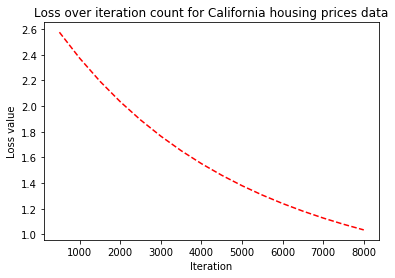
\includegraphics[scale=0.5]{cali.png}
    \caption{Loss function over iterations for California housing prices dataset}
    \label{fig:leastsq:1}
\end{figure}

\subsection{Binary classification experiments}
For classification, our experiments were conducted by running gradient descent for a fixed number of iterations, and then comparing various classification metrics over the two learning rates.

\begin{table}
    \caption{Binary classification experiments on various datasets with $\alpha=0.1$ and $\alpha=\frac{1}{L}$}
    \centering
    \begin{tabularx}{\textwidth}{cYYYY}
        \toprule
        Dataset & \# iterations & Inverse Lipschitz constant & Cost with $\alpha=0.1$ & Cost with $\alpha=\frac{1}{L}$ \\
        \midrule
        Iris & 1,000 & 70.54 & 0.6928 & 0.284 \\
        Covertype & 1,000 & 42,021.68 & 0.69315 & 0.6905 \\
        \bottomrule
    \end{tabularx}
    \label{tab:classif:1}
\end{table}

\begin{itemize}
    \item binary loss (logistic reg): census income
    \item format wants line after the table heading
    \item softmax: MNIST, iris
    \item Todo: check derivation for softmax, whether it is $\left\Vert X \right\Vert$ or $\left\Vert y^T X \right\Vert$.
    \item don't set threshold...run for certain iterations..capture MSE comparison every 100 iterations, may be
    \item CI of regression coefficients
    \item SVM analogy
\end{itemize}
\bibliographystyle{plain}
\bibliography{cite}
\end{document}
